% --- SEKTION 1: SYSTEMKOMPONENTEN UND STEUERUNG ---

\section{Systemkomponenten (SCS)}
Il \textbf{System Control Space (SCS)} gestisce le funzioni principali del processore, inclusa la configurazione dell'NVIC e dei System Control Registers.

\subsection{Fault- und Ausnahmemechanismen}
\begin{itemize}
    \item \textbf{HardFaults:} Sempre attivi; gestiscono errori di Bus, Usage e Memory-Management.
    Consentono una rapida reazione a errori critici.
    \item \textbf{Wake-up Interrupt:} Consente la disattivazione gerarchica dei componenti
     per ridurre il consumo energetico (modalità Sleep/Stop).
    \item \textbf{Memory Protection Unit (MPU):} Genera eccezioni in caso di accessi alla memoria non autorizzati.
    \item \textbf{Debug Unit:} Fornisce fino a 4 hardware-breakpoints per il debug del codice.
\end{itemize}

\subsection{System Tick Timer (SysTick)}
Un contatore \textbf{24-bit}, che fornisce una base temporale costante per il sistema operativo o per l'esecuzione dei programmi.

\section{Stack und Speicherverwaltung}
Lo \textbf{stack} è una memoria temporanea, utilizzata per le variabili locali e per il salvataggio del contesto durante le eccezioni.

\begin{itemize}
    \item \textbf{Direzione:} Cresce verso indirizzi di memoria più bassi.
    \item \textbf{Stack Pointer (SP):} Indica sempre il "top of stack".
    È vietato leggere o scrivere al di sotto di SP.
    \item \textbf{Allineamento:} Normalmente assegnato a passi di 8 byte.
    \item \textbf{Velocità:} Circa il doppio rispetto al puntatore RAM/ROM, poiché (SP) è già disponibile.
\end{itemize}

\section{Interrupt-Verwaltung (NVIC)}

\begin{itemize}
    \item Il \textbf{Nested Vector Interrupt Controller} gestisce la priorità e il passaggio tra il programma in background e la \textbf{Interrupt Service Routine (ISR)}.
    \item \crd{Il LSB in ogni vettore indica la modalità di salto (1: thumb, 0: ARM) nel Cortex-M; nel Cortex-M è sempre 1} (Anche gli indirizzi in \texttt{LR} con \texttt{B..})
    \item In genere, la VT (vector table) viene salvata in memoria tra il codice di boot e la seconda istruzione.
    \item Tramite VTOR (Vector Table Offset Register) è possibile modificare la posizione della tabella in memoria.
    \item \textbf{Stati degli interrupt:} \textit{Pending} (richiesto dalla periferia, resettato automaticamente dall'hardware al momento dell'ingresso nella ISR), \textit{Active} (in esecuzione nel Handler Mode), \textit{Inactive}.
\end{itemize}

\subsection{NVIC Special Features}
\begin{itemize}
    \item \textbf{Tail-Chaining:} L'IRQ a priorità più bassa è ancora pending alla fine della ISR,
    quando una ISR attiva termina, la CPU salta oltre Unstacking e Stacking.
    Esegue solo un nuovo Vector Fetch
    (da 15 $\rightarrow$ passaggio da soli \textbf{6 cicli}).
    \item \textbf{Late Arrival:} Un IRQ a priorità alta viene attivato durante lo stacking di un IRQ a priorità bassa,
    la CPU completa lo stacking, ma esegue direttamente il Vector Fetch dell'IRQ più urgente.
    \item \textbf{Pop-Preemption:} Un IRQ arriva durante il final Unstacking (Pop); l'hardware lascia il Pop e passa immediatamente alla nuova ISR, in soli \textbf{6 cicli}.
\end{itemize}

\begin{minipage}[t]{0.51\columnwidth}
    \subsection{Maskierungsregister}
    \begin{itemize}
        \item \textbf{PRIMASK:} 1 bit.
        Disabilita tutti gli interrupt programmabili (eccetto HardFault e NMI).
        \item \textbf{FAULTMASK:} 1 bit. Disabilita gli interrupt e tutte le eccezioni (eccetto NMI).
        \item \textbf{BASEPRI:} Disabilita gli interrupt con priorità numerica maggiore o uguale (minore urgenza) a un valore impostato.
    \end{itemize}
    
    \subsection{Latenza e Stacking}
    \begin{itemize}
        \item \textbf{Interrupt Latency:} Tempo fisso fino all'ingresso nella ISR senza overhead software.
        \textbf{Cortex-M0+:} 15--16 cicli di clock. \textbf{Cortex-M3/M4:} 12 cicli.
        \item Le funzioni della ISR sono del tipo \texttt{void ISR\_Handler(void)}: accettano nessun parametro e non restituiscono valori.
    \end{itemize}
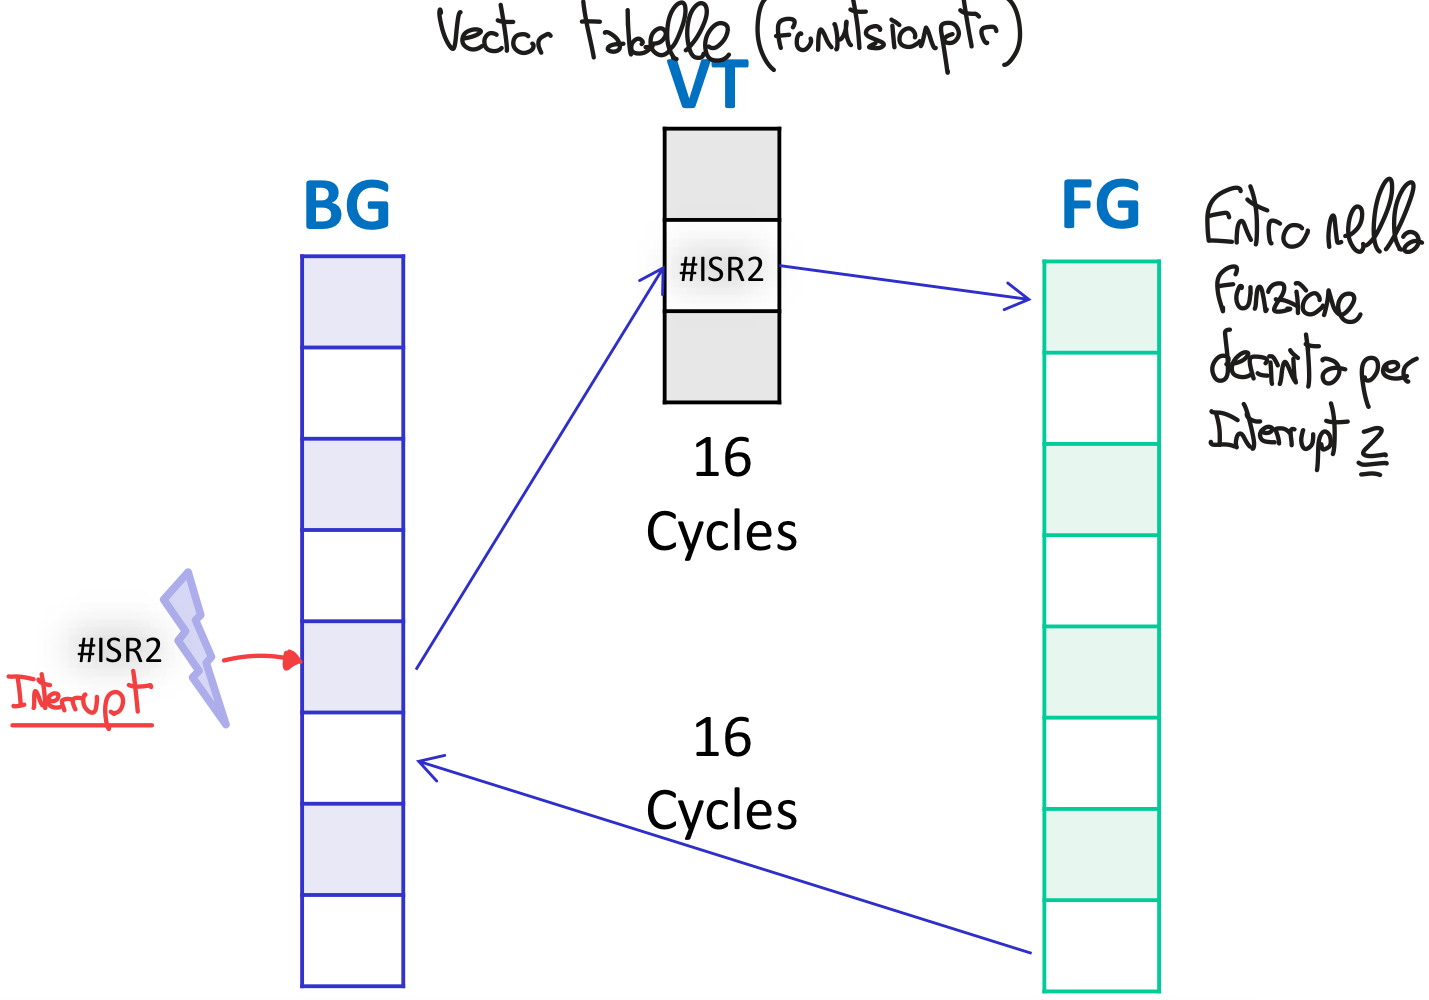
\includegraphics[width=\linewidth]{images/NVIC_sequence.png}
\end{minipage}
\hfill
\begin{minipage}[t]{0.47\columnwidth}
    \subsection{Preemption vs Subpriority}
    \begin{itemize}
        \item \textbf{Cortex-M0+:} Supporta solo 2 bit di priorità, utilizzabili solo come preemption.
        \item \textbf{Cortex-M3/M4:} Tramite \textit{Priority Grouping} gli 8 bit di priorità vengono suddivisi in:
        \begin{itemize}
            \item \textbf{Preemption bits:} Decidono se un interrupt può interrompere una ISR fisicamente in esecuzione (\textit{nesting}).
            \item \textbf{Subpriority bits:} Criterio per la risoluzione temporale quando due IRQ arrivano contemporaneamente
        \end{itemize}
    \end{itemize}
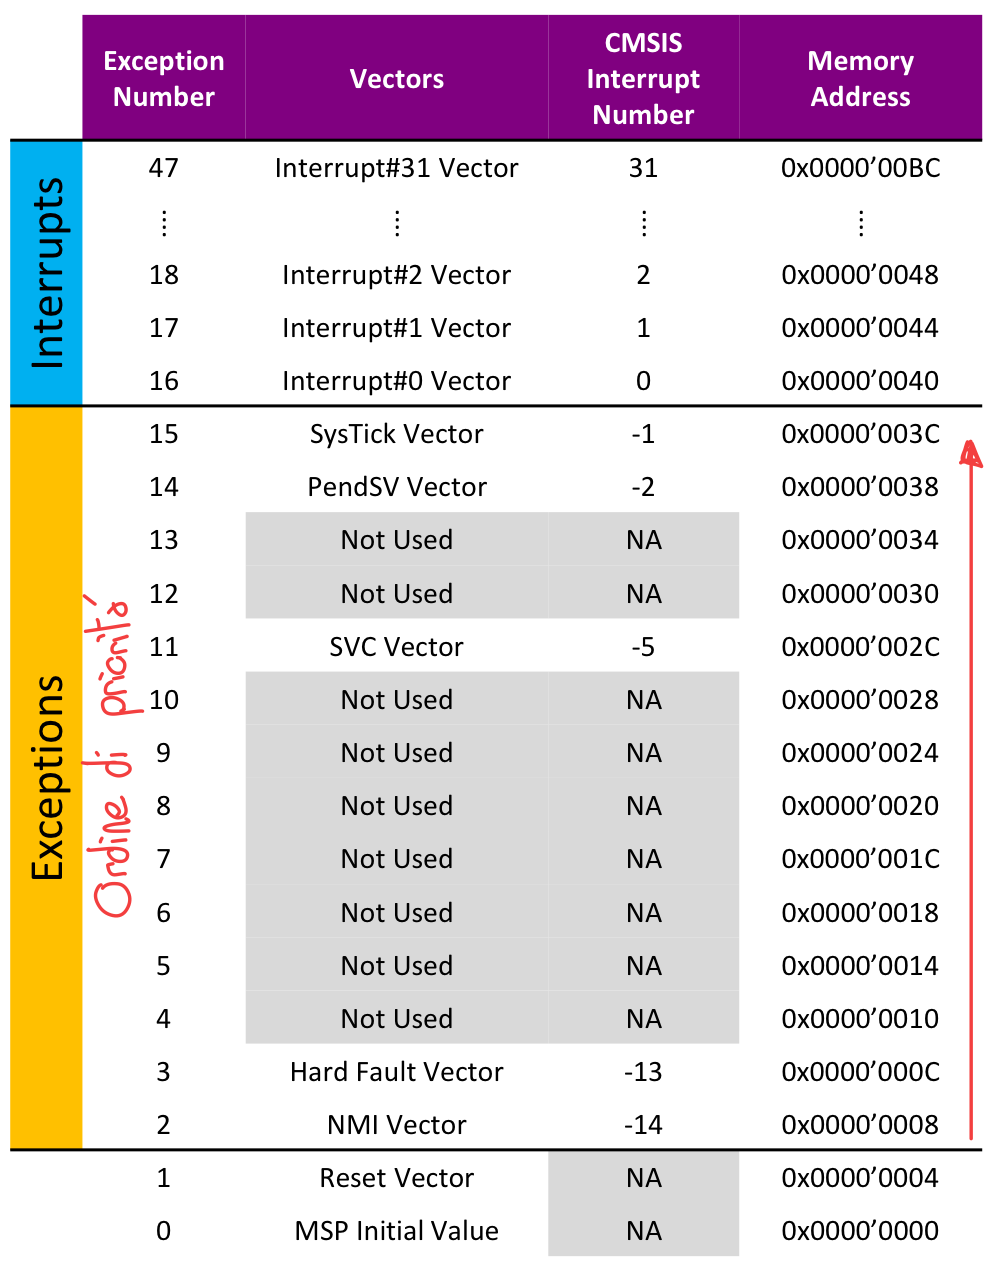
\includegraphics[width=\linewidth]{images/NVIC_table.png}
\end{minipage}

\subsection{Alternative Lösungen \& IRQ-Signale}
\begin{minipage}{0.55\columnwidth}
    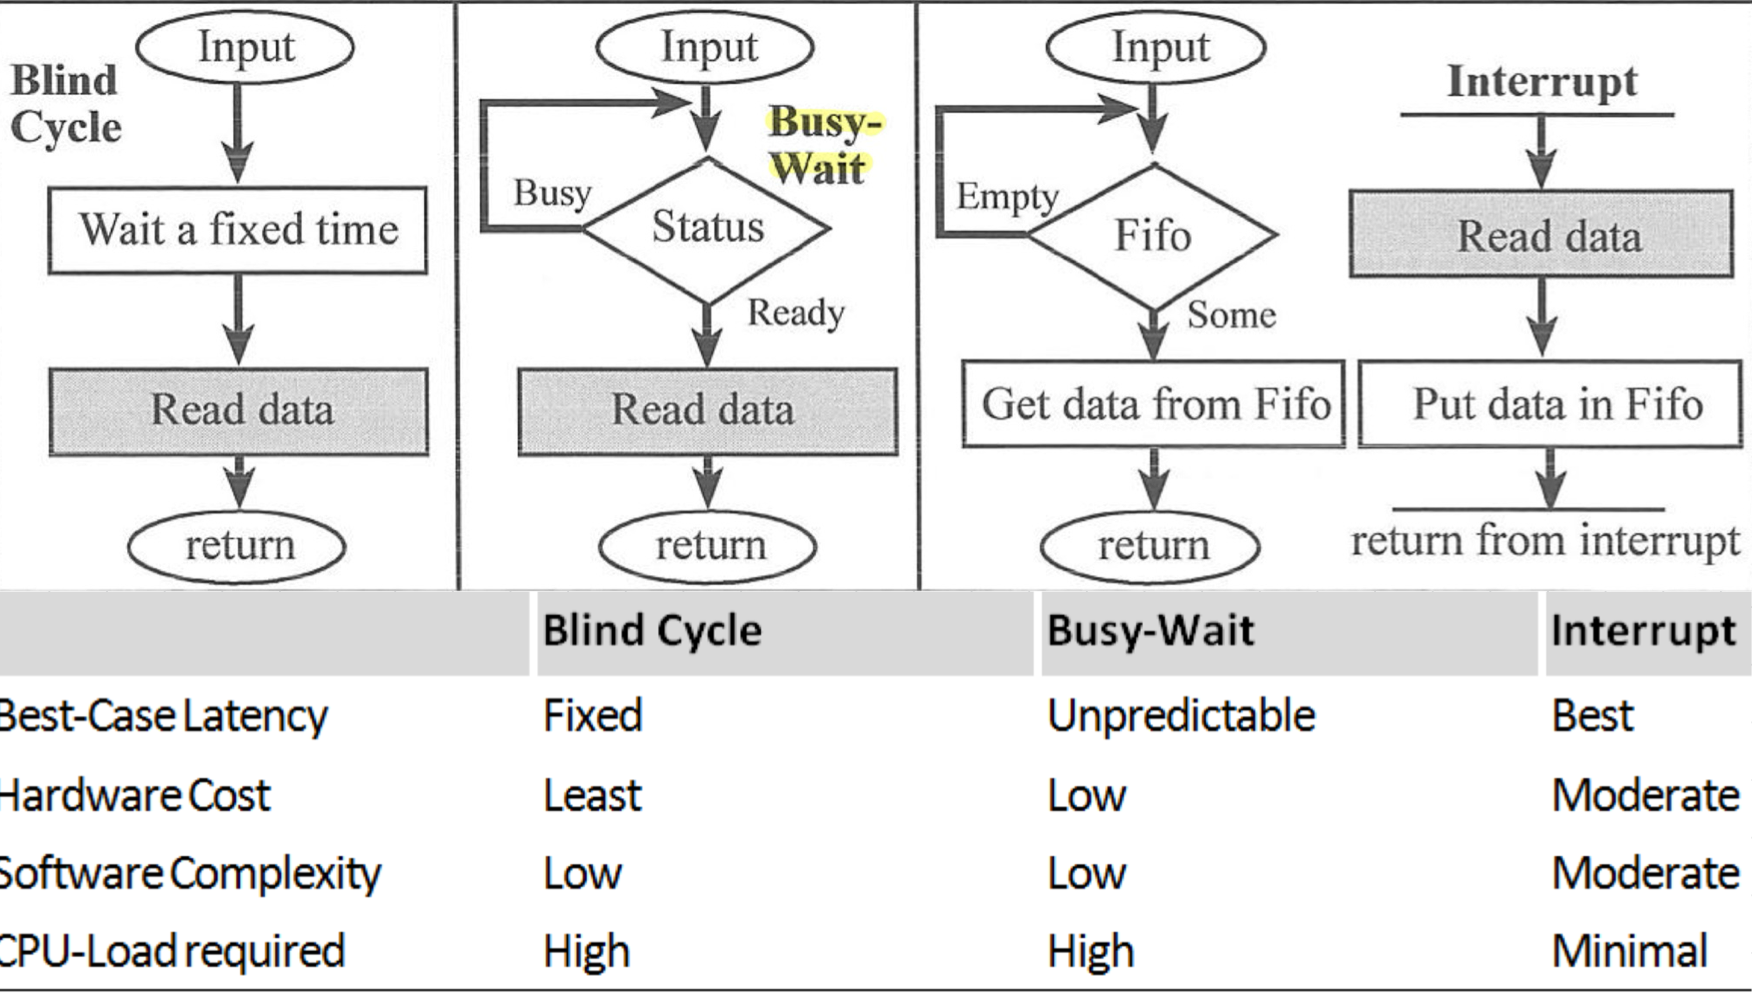
\includegraphics[width=\linewidth]{images/pooling_interrupts.png}
\end{minipage}
\begin{minipage}{0.45\columnwidth}
    \begin{enumerate}
        \item \textbf{Software Clearing}
        \item \textbf{Software Clearing con Reset}
        \item \textbf{ISR Reentry (IRQ pulsato durante la ISR)}
        \item \textbf{Repulsed IRQ}
        \item \textbf{Pulsed IRQ (il livello rimane attivo)}
    \end{enumerate}
\end{minipage}

% Erste Bildreihe
\begin{minipage}[b]{0.5\linewidth}
    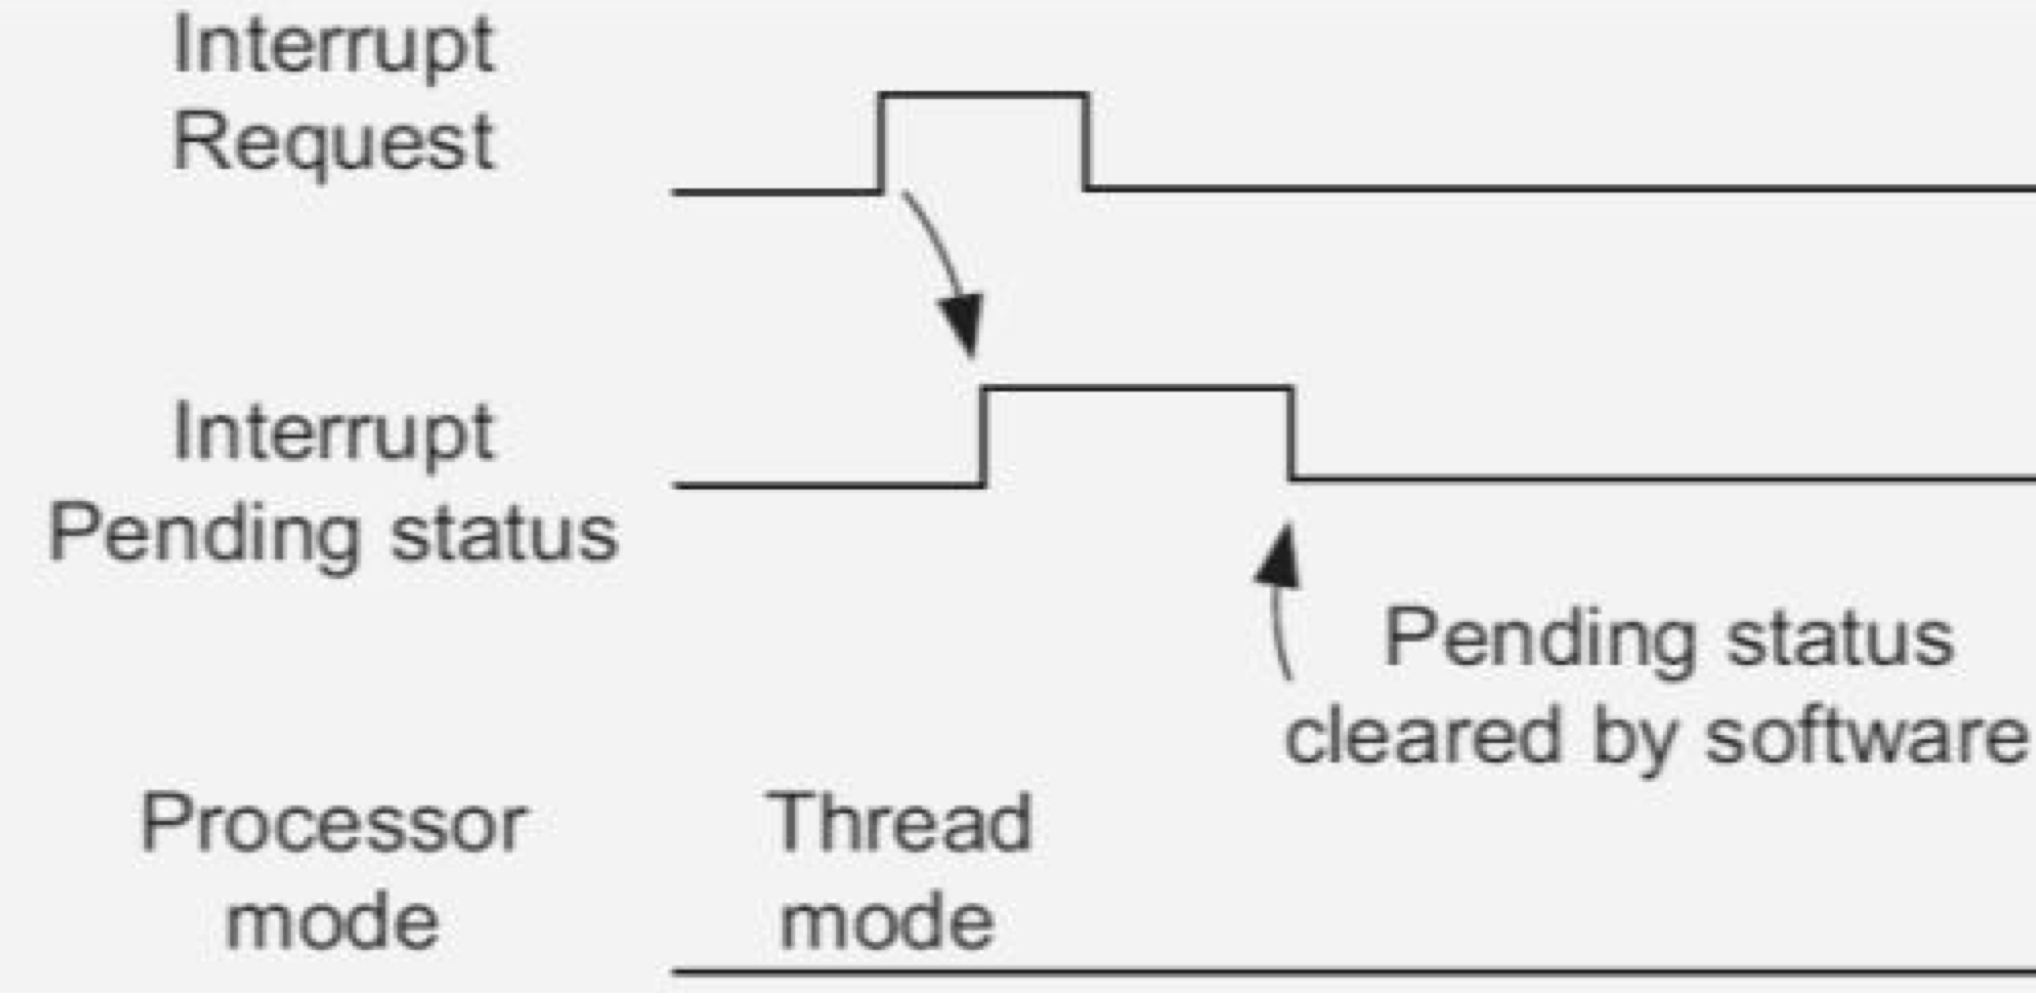
\includegraphics[width=0.8\linewidth]{images/software_clearing.png}
\end{minipage}
\begin{minipage}[b]{0.5\linewidth}
    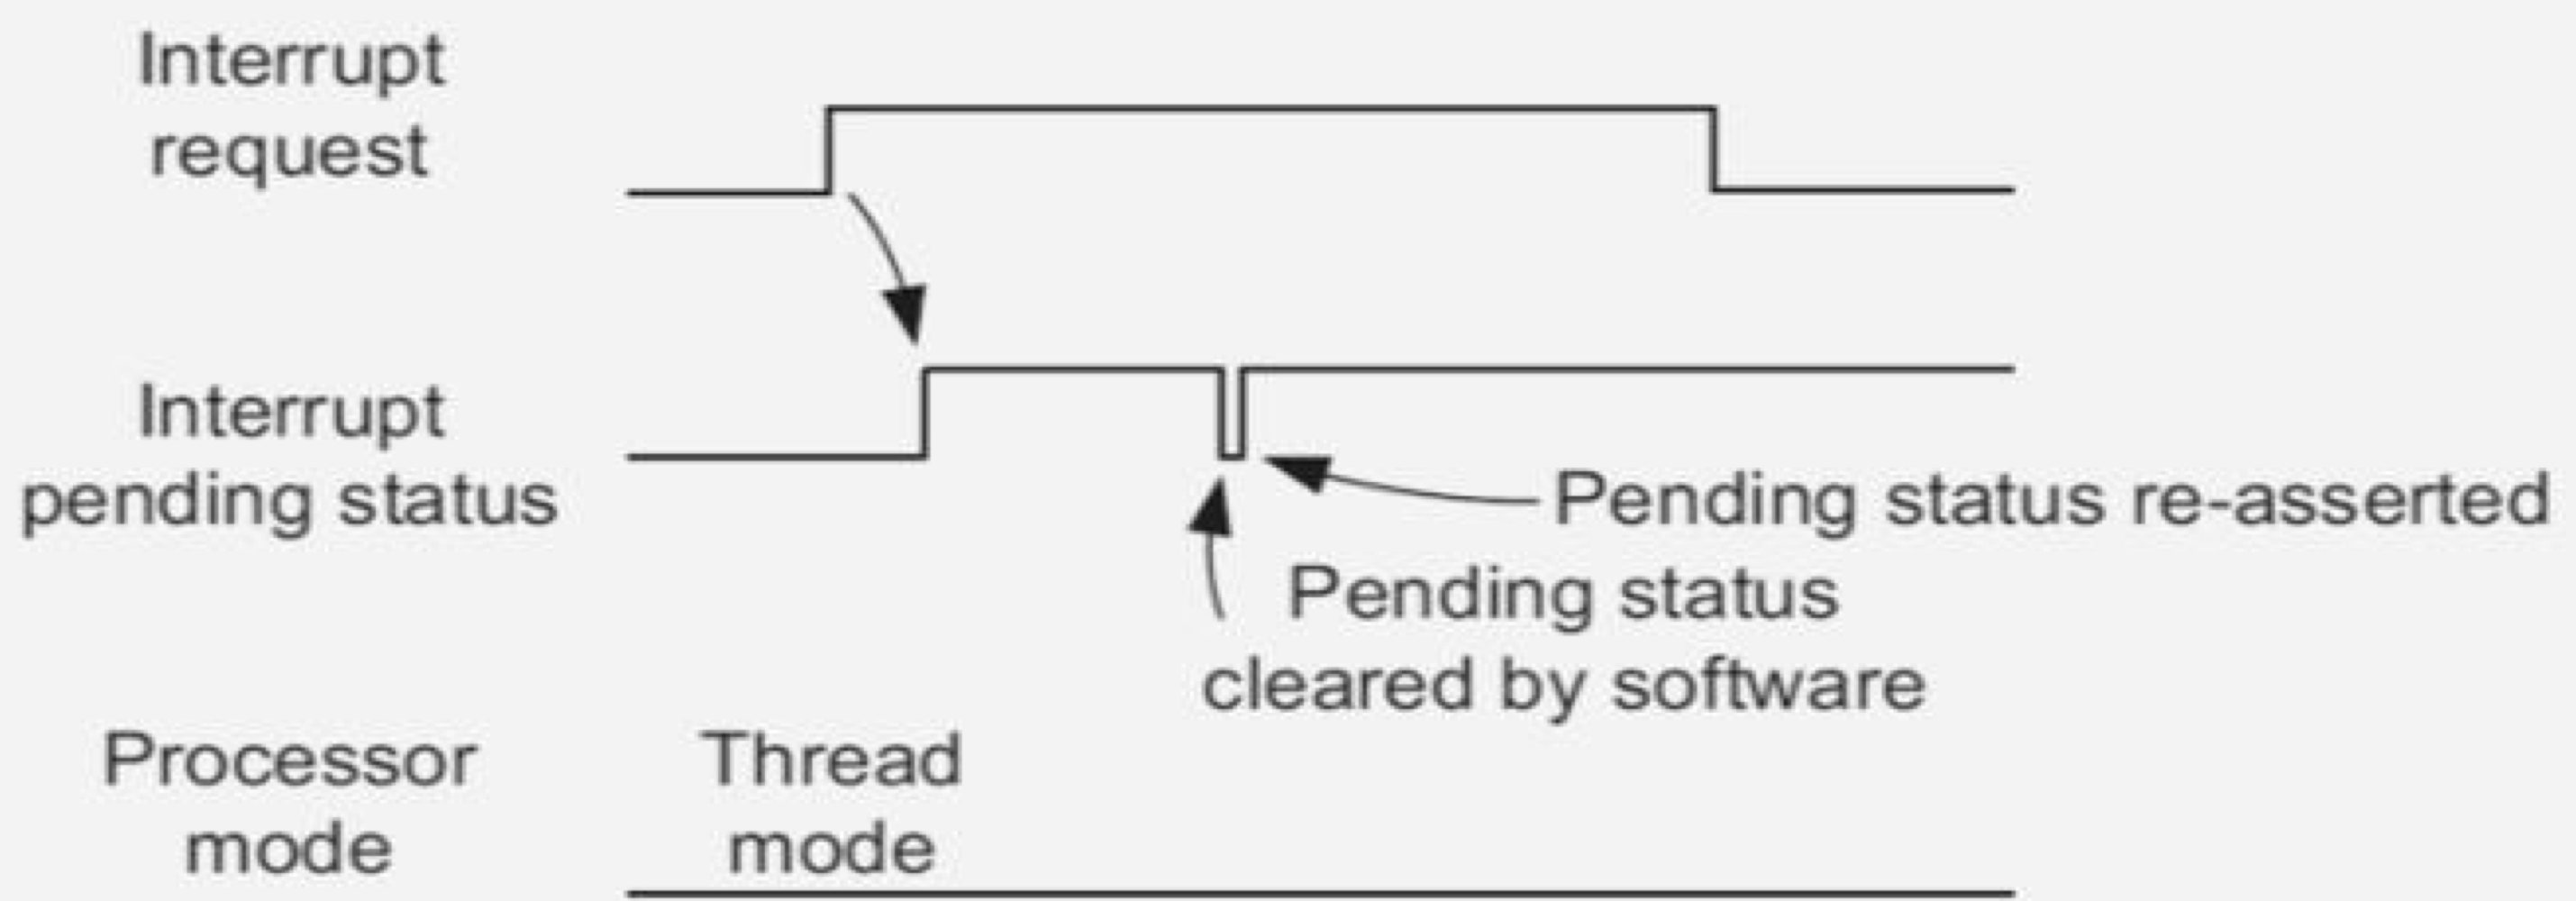
\includegraphics[width=\linewidth]{images/software_clearing_reset.png}
\end{minipage}

% Zweite Bildreihe
\begin{minipage}[b]{0.5\linewidth}
    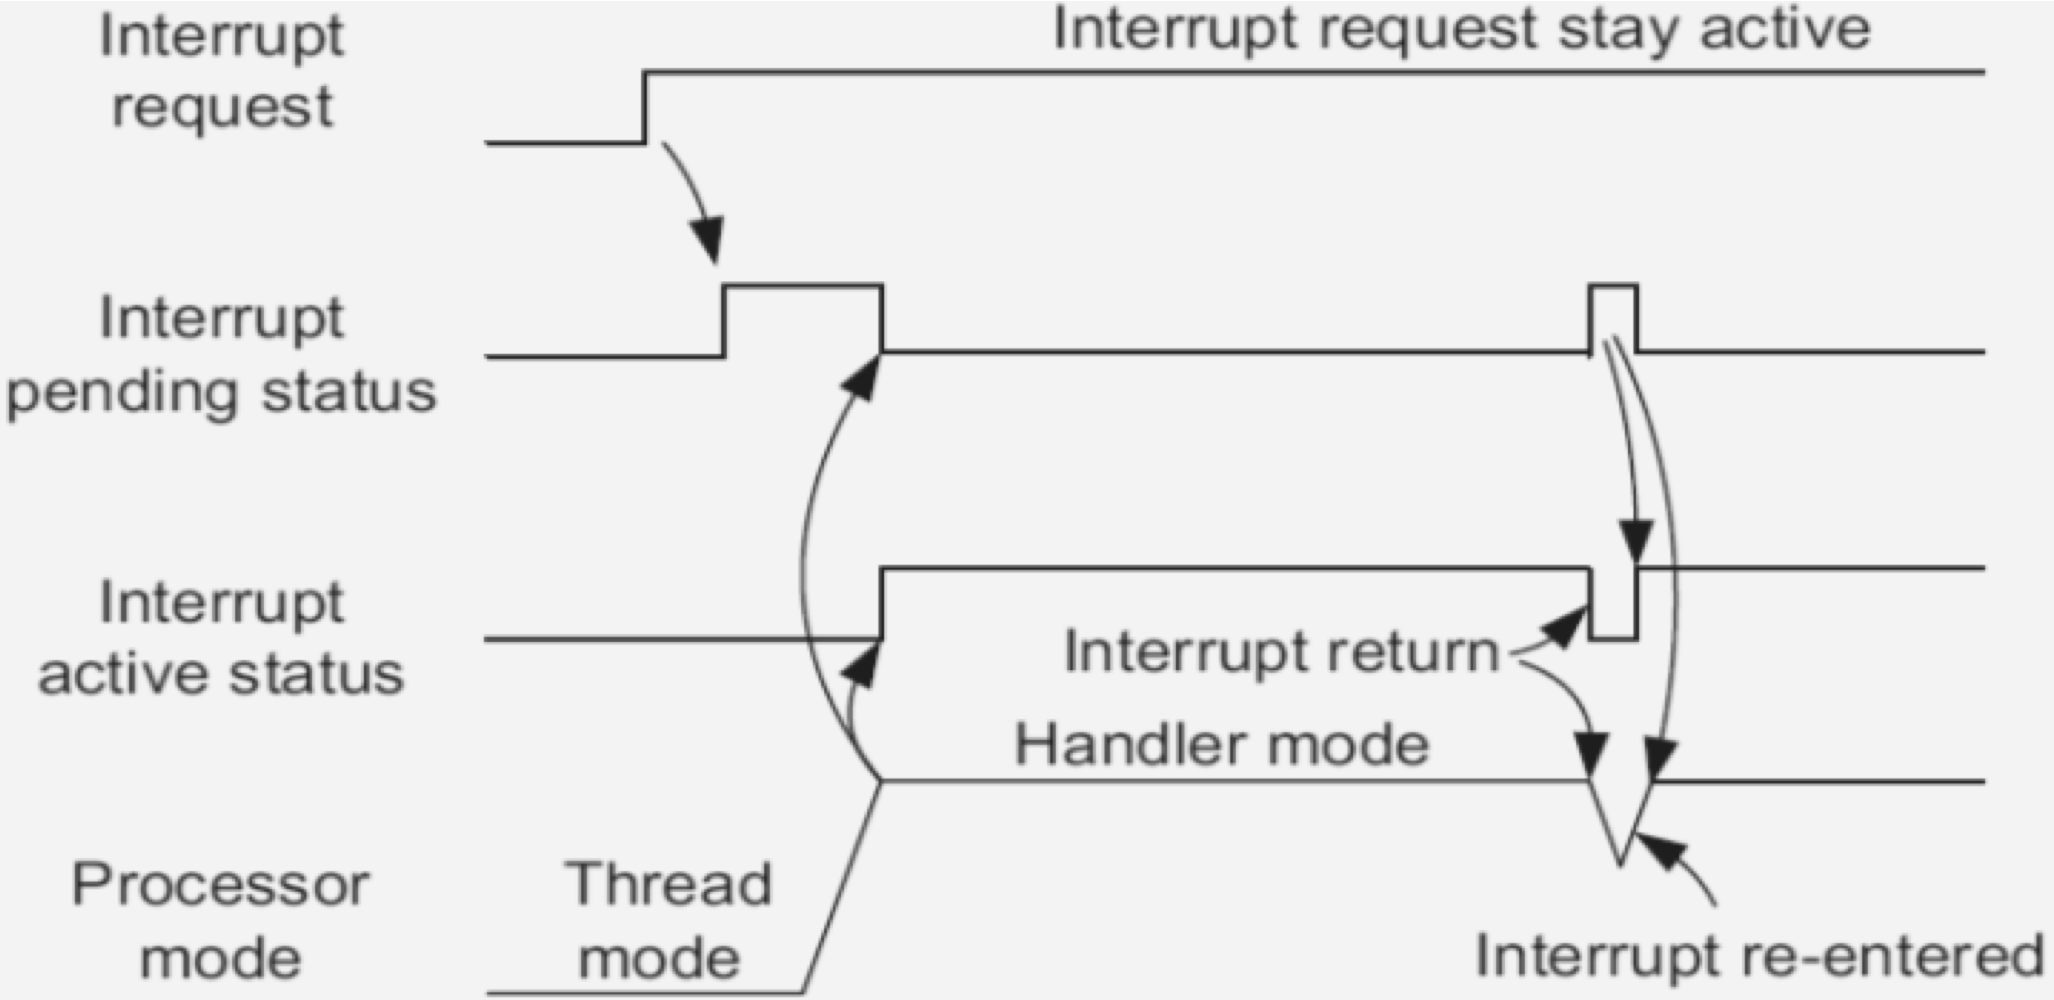
\includegraphics[width=\linewidth]{images/isr_reentry.png}
\end{minipage}
\begin{minipage}[b]{0.5\linewidth}
    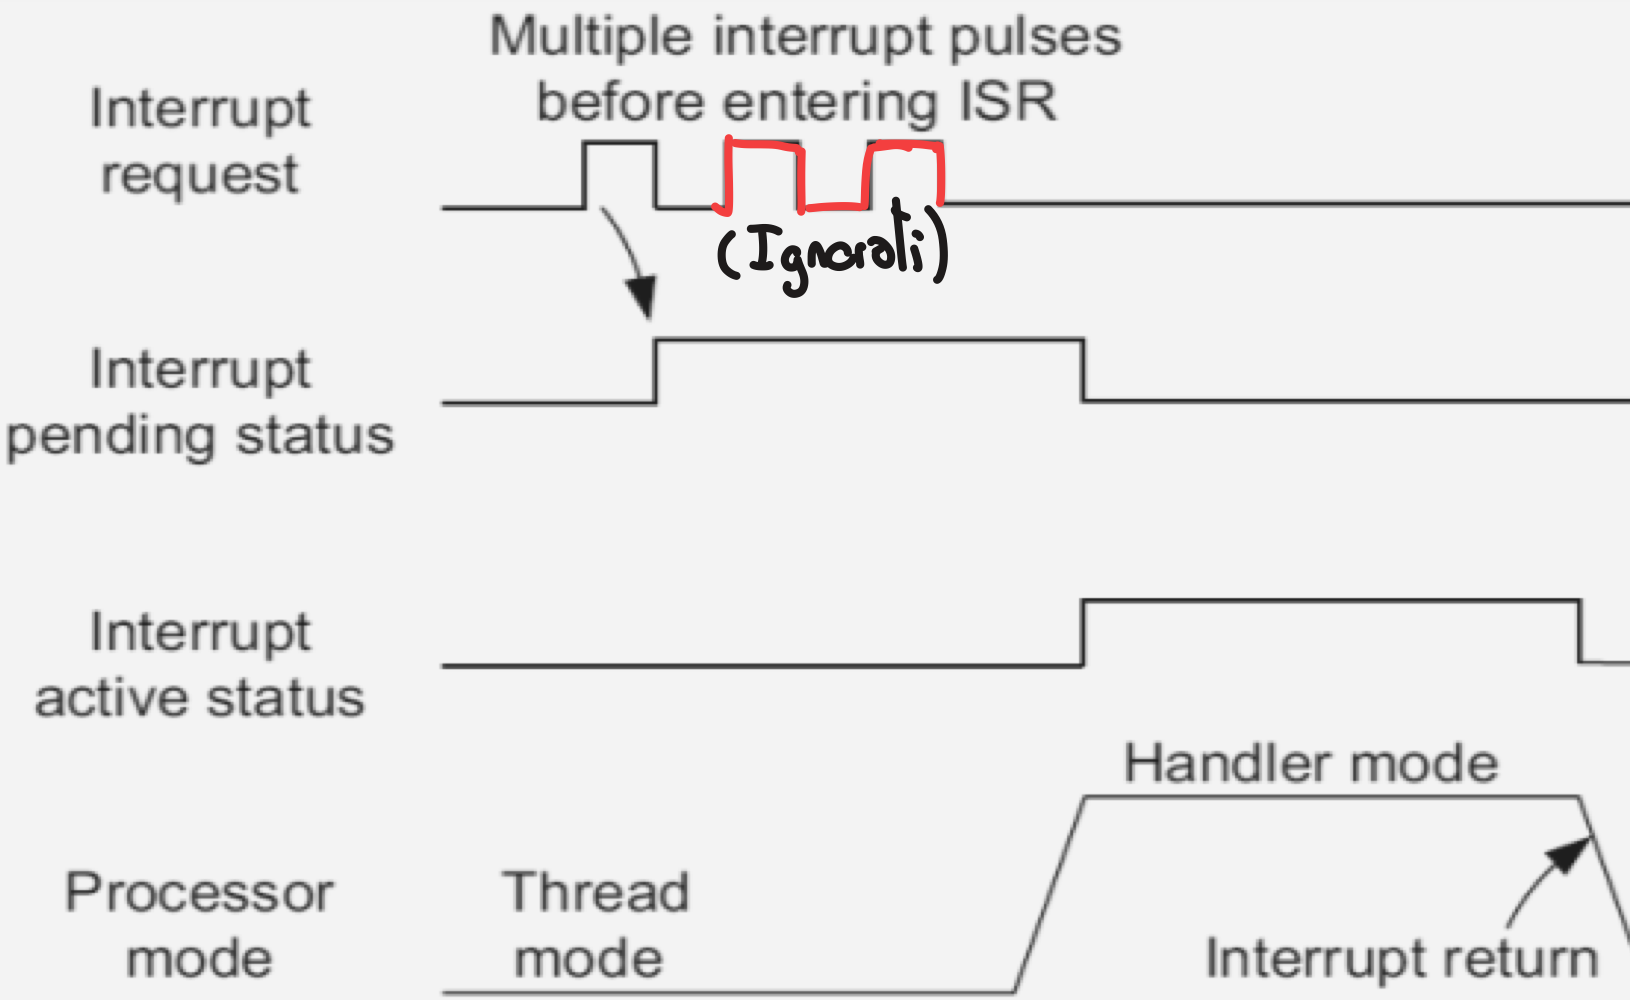
\includegraphics[width=0.9\linewidth]{images/repulsed_irq.png}
\end{minipage}

% Dritte Reihe (letztes Bild zentriert oder links)
\begin{minipage}[t]{0.5\linewidth}
    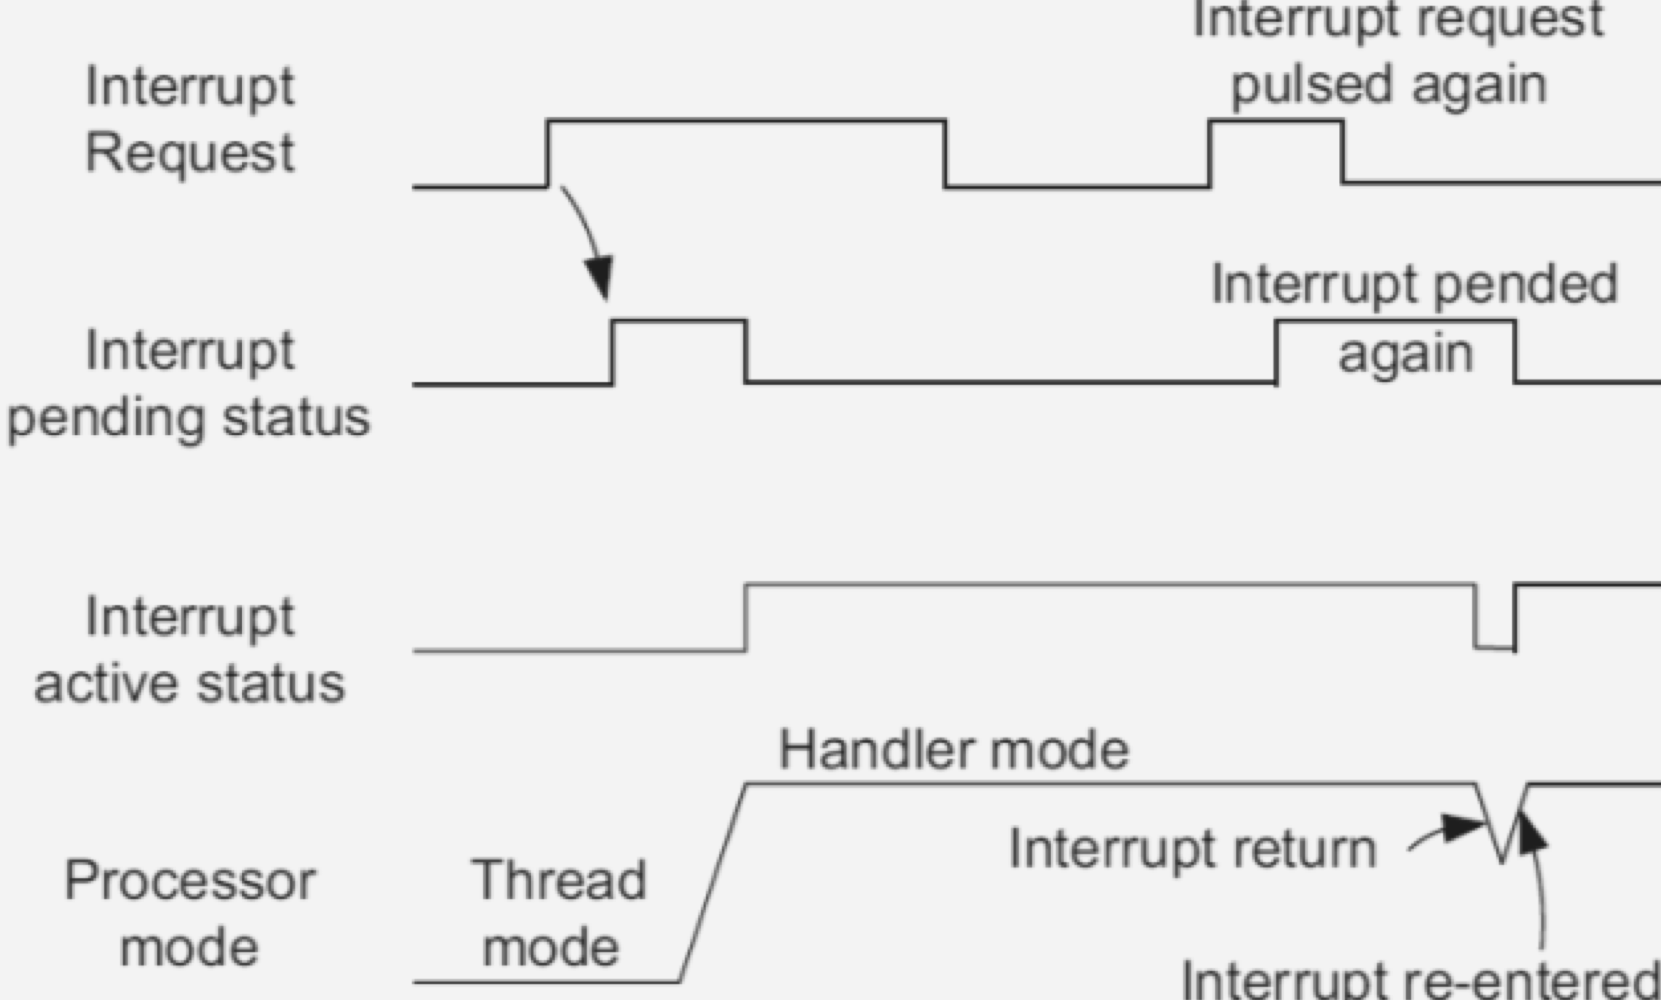
\includegraphics[width=\linewidth]{images/pulsed_irq.png}
\end{minipage}